\section{Ricerca in un array}

{\textbf{Input:}} array $A$, elemento $x$\\
{\textbf{Output:}} 
\begin{itemize}
    \item indice $i$ t.c. $A[i]$ = $x$
    \item -1 se $A$ non contiene $x$
\end{itemize}

\subsection{Ricerca sequenziale}
\begin{figure}[h]
    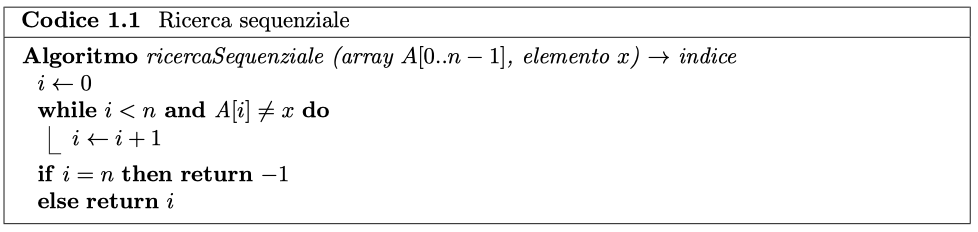
\includegraphics[width=\textwidth]{1-1.png}
    \centering
\end{figure}

\noindent Posso rendere l'algoritmo più "intelligente" cercando a partire dal fondo.
In questo modo se l'elemento non è nell'array l'indice diventa automaticamente -1.
\begin{figure}[h]
    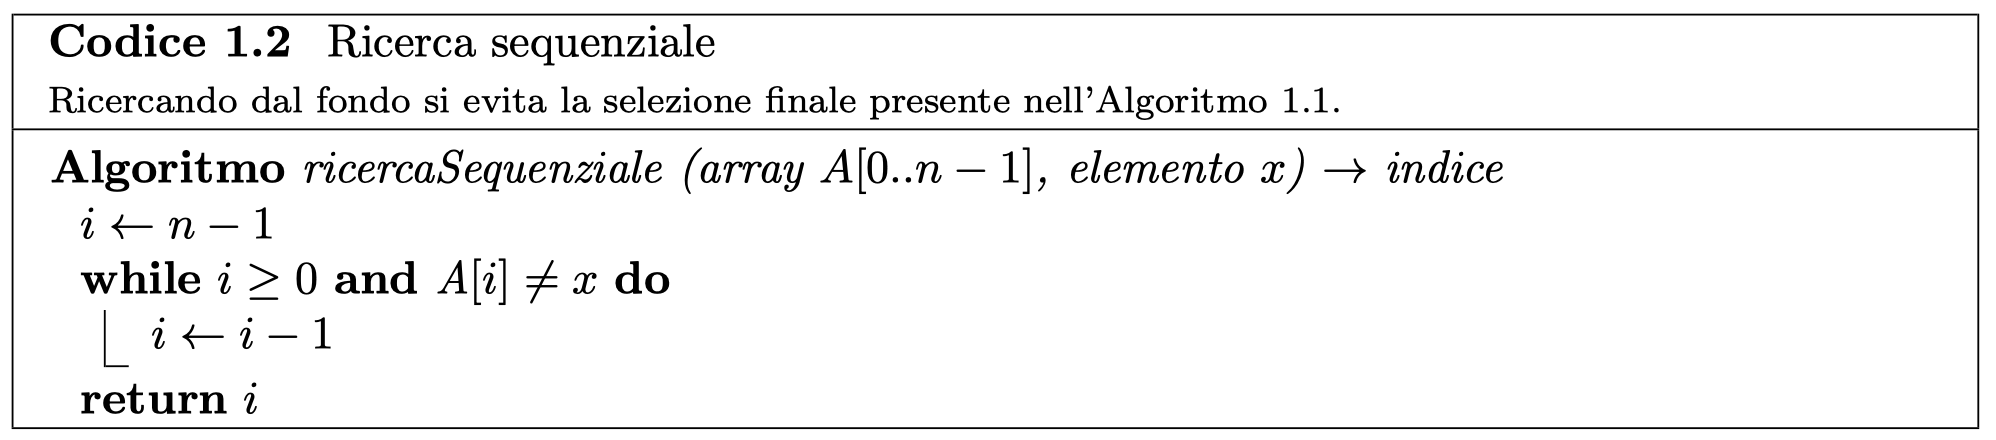
\includegraphics[width=\textwidth]{1-2.png}
    \centering
\end{figure}

\noindent {\textbf{Tempo:}} $\Theta(n)$
\clearpage

\subsection{Ricerca binaria o dicotomica}
Se ho un array ordinato posso usare un algoritmo di ricerca binaria.

\begin{figure}[h]
    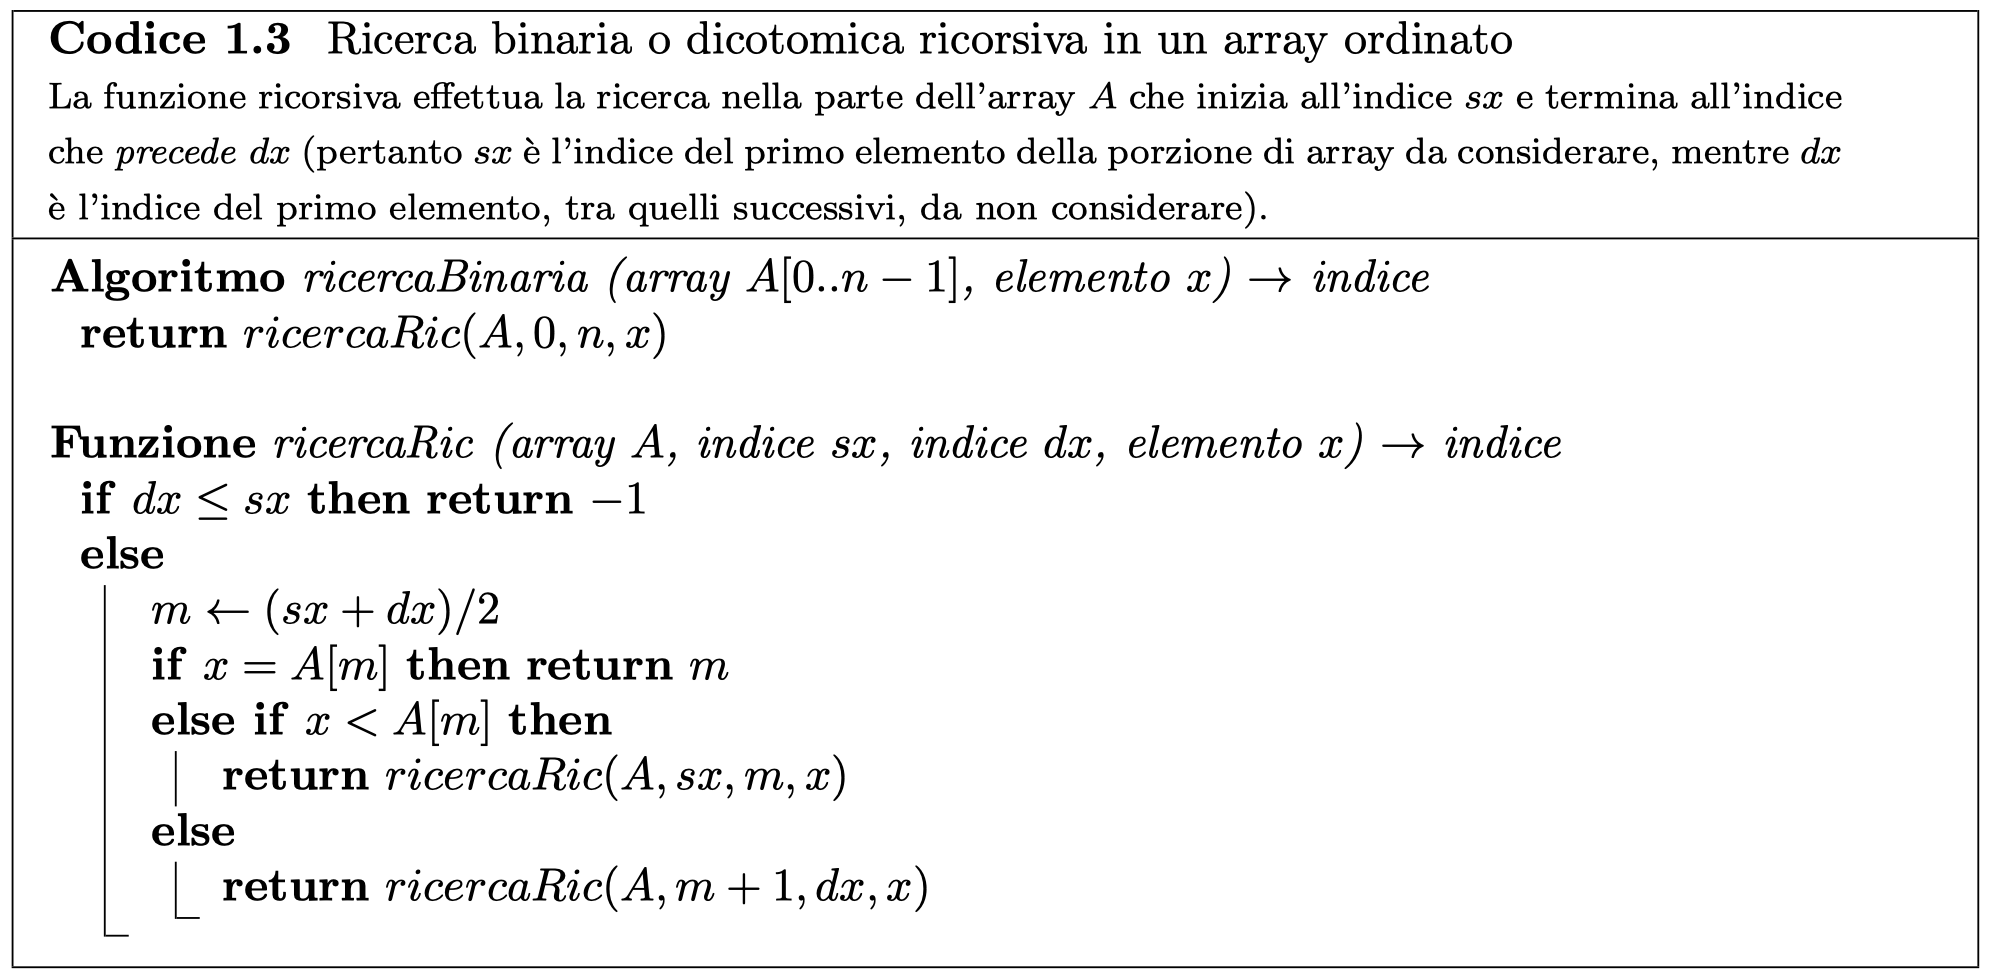
\includegraphics[width=\textwidth]{1-3.png}
    \centering
\end{figure}

\begin{figure}[h]
    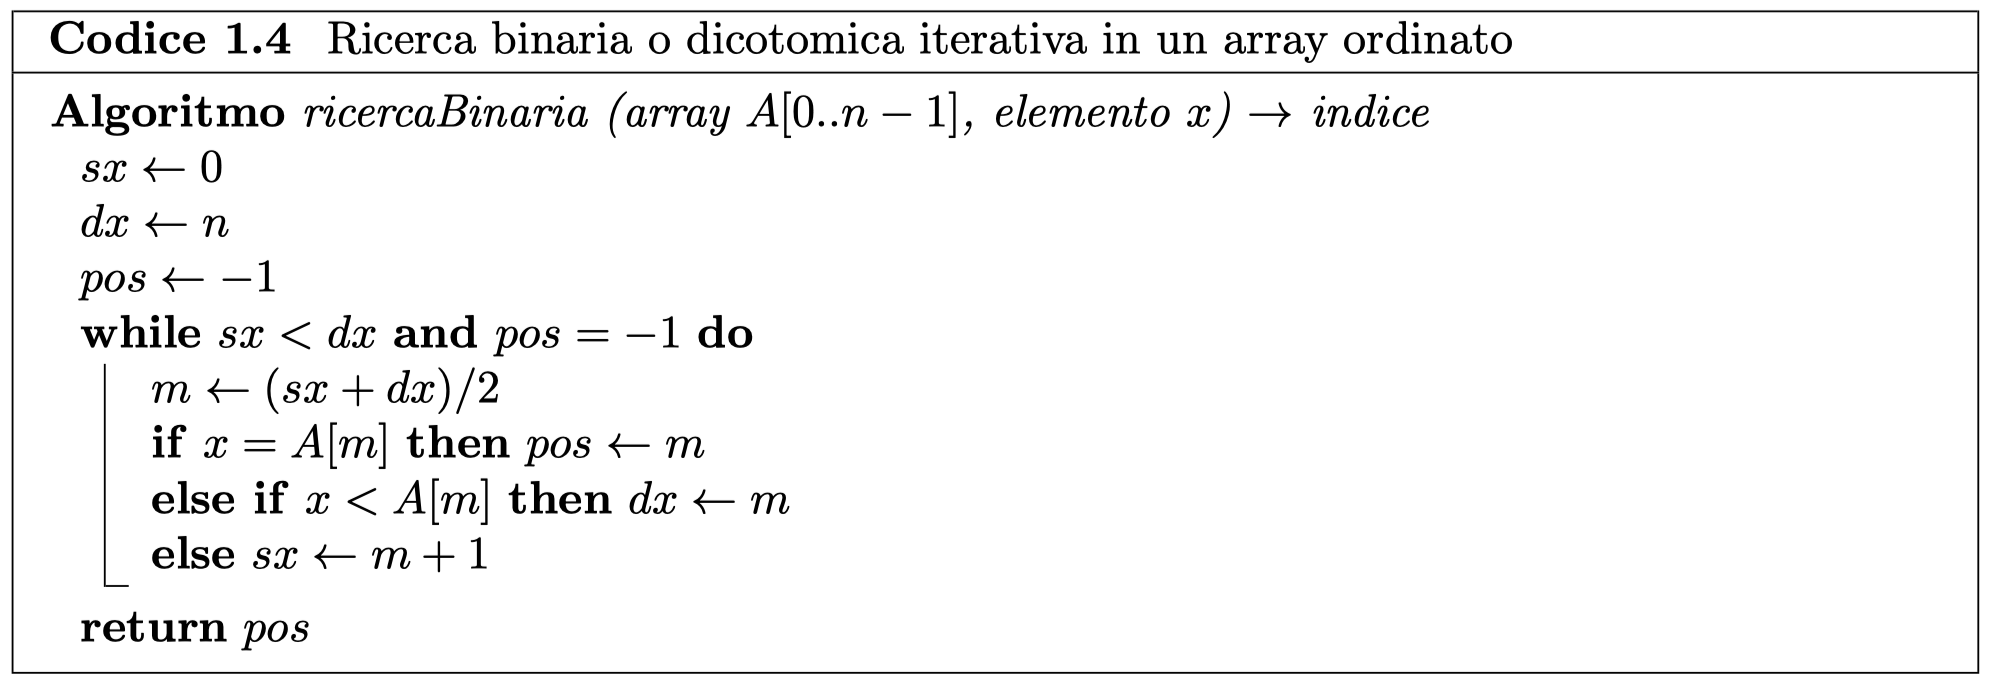
\includegraphics[width=\textwidth]{1-4.png}
    \centering
\end{figure}
\clearpage

\subsubsection{Alcune note sullo pseudocodice}
\begin{itemize}
    \item {\emph{Indici degli array}}\\
    Quando si definisce un array (in questo caso nei parametri degli algoritmi o della funzione), 
    il range di indici viene indicato qualora sia rilevante per la scrittura dell’algoritmo. 
    Quando non sia rilevante o sia chiaro dal contesto, il range viene omesso 
    (come, in questo esempio, per il parametro A della funzione ricercaRic).

    \item {\emph{Operatori logici}}\\
    Assumiamo che per congiunzione ({\emph{and}}) e disgiunzione ({\emph{or}}) sia utilizzata la 
    {\emph{lazy-evaluation}}. Pertanto in una condizione della forma 
    $a$ {\textbf{and}} $b$ la condizione $b$ viene valutata solo se $a$ è vera, 
    mentre in una condizione della forma $a$ {\textbf{or}} $b$ la seconda viene valutata solo se $a$ è falsa.

    \item {\emph{Passaggio di parametri}}\\
    Assumiamo che per i tipi semplici il passaggio di parametro avvenga sempre
    {\emph{per valore}} mentre per i tipi strutturati avvenga il passaggio {\emph{per riferimento}}.

    
\end{itemize}

\clearpage